\documentclass{cmn}

\def\cellWidth{9mm}
\def\cellHeight{6mm}
\def\numCells{4}
\def\textWidth{40mm}

\begin{document}
  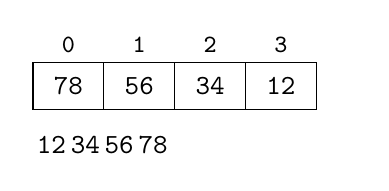
\begin{tikzpicture}
    \pgfmathsetmacro{\lastIndex}{\numCells-1}

    \draw (0,0) -- ++(\numCells*\cellWidth,0) -- ++(0,\cellHeight) -- ++(-\numCells*\cellWidth,0) -- cycle;
    \foreach \i in {1,...,\lastIndex} {
      \draw (\i*\cellWidth,0) -- ++(0,\cellHeight);
    }
    \foreach \i/\t in {1/78,2/56,3/34,4/12} {
      \node at (\i*\cellWidth-0.5*\cellWidth,0.5*\cellHeight) {\texttt{\t}};
    }
    \foreach \i in {0,...,\lastIndex} {
      \node at (\i*\cellWidth+0.5*\cellWidth,1.375*\cellHeight) {\small\texttt{\i}};
    }

    \node[text width=\textWidth,align=left] at (0.5*\textWidth+0.5mm,-0.75*\cellHeight) {\texttt{12\,34\,56\,78}};
  \end{tikzpicture}
\end{document}
